\chapter{Adapting Latent Dirichlet Allocation to Overlapping Community Detection}
\doublespacing
\label{chap:lda}
\minitoc

\section{Introduction to the Latent Dirichlet Allocation Adaptation}
In Natural Language Processing (NLP), Latent Dirichlet Allocation (LDA) \cite{blei2003latent} is a classical document clustering method, a Bayesian network that models how documents in a corpus are topically related.
It is used to detect latent topics from documents by constructing a three-layer probabilistic graphical model: document-topic-word. In this three-layer model, documents and words can be observed from a dataset, while topics are a hidden layer which has to be estimated from the observed data.  
In StackOverflow, a user submits a question, then assigns 1$\sim$5 tags to indicate the key topics touched by this question. Other users who are interested in the question may provide answers to the question or comment on the question or others' answers. Therefore the main structuring graph in StackOverflow is the question-answer graph. As tags attached to a question  reflect its scope and domain, users answering a question can be considered as interested by this domain. As a result, a first approach is to consider that a user answering a question acquires the tags attached to this question and gradually, each user acquires a list of tags associated with frequencies. If we treat a user as a document and tags acquired by the user as words in a document, then community detection can be considered as a clustering problem where users with similar topics of interest are grouped into the same cluster forming a community of interest.

Similarly to \cite{Li:2010:CTM:1871437.1871673}, we applied the classic LDA method to construct a users-topics-tags model to detect latent topics of interest from the tags acquired by users and then cluster users into different topics. The output of the model consists of two probability distributions:
\begin{enumerate}
 \item a User-Topic distribution to describe to what extent a user is interested in the different topics.
 \item a Topic-Tag distribution to describe to what extent a topic is related the different tags.
\end{enumerate}



The formalization of this model is given by equation~\ref{eq:general}: 
\begin{equation}
P(t|u)=P(t|z)*P(z|u)
\label{eq:general}
\end{equation}
where $t$ denotes a tag, $z$ denotes a latent topic, $u$ denotes a user. The probability of a tag for a user is the result of multiplying the probability of this tag for a topic and the probability of this topic for the user.

%TODO: Fab: I changed the text below please check it is correct
Probabilistic graphical models (PGM) express the conditional dependence structure between random variables as a graph. 
The plate notation of the PGM of our model is presented in Figure \ref{fig:lda}. 
The variables appear as blue disks if the variable is observed and white disks if the variable is hidden (guessed).
The dependencies among the variables are captured by the direction of the edges. 
The boxes represent replicated variables, which are users, topics (interests) and tags. The outer boxes represent users, while the inner boxes represent the repeated choice of topics and tags for a user. The parameters of this model are explained in Table \ref{tab:parameters}.
$M$ and $V$ are given while $K$, $\alpha$ and $\beta$ can be chosen. $T$ is observed through the users' tag lists. Other variables are latent variables which have to be estimated.

\begin{figure}[htbp]\centering
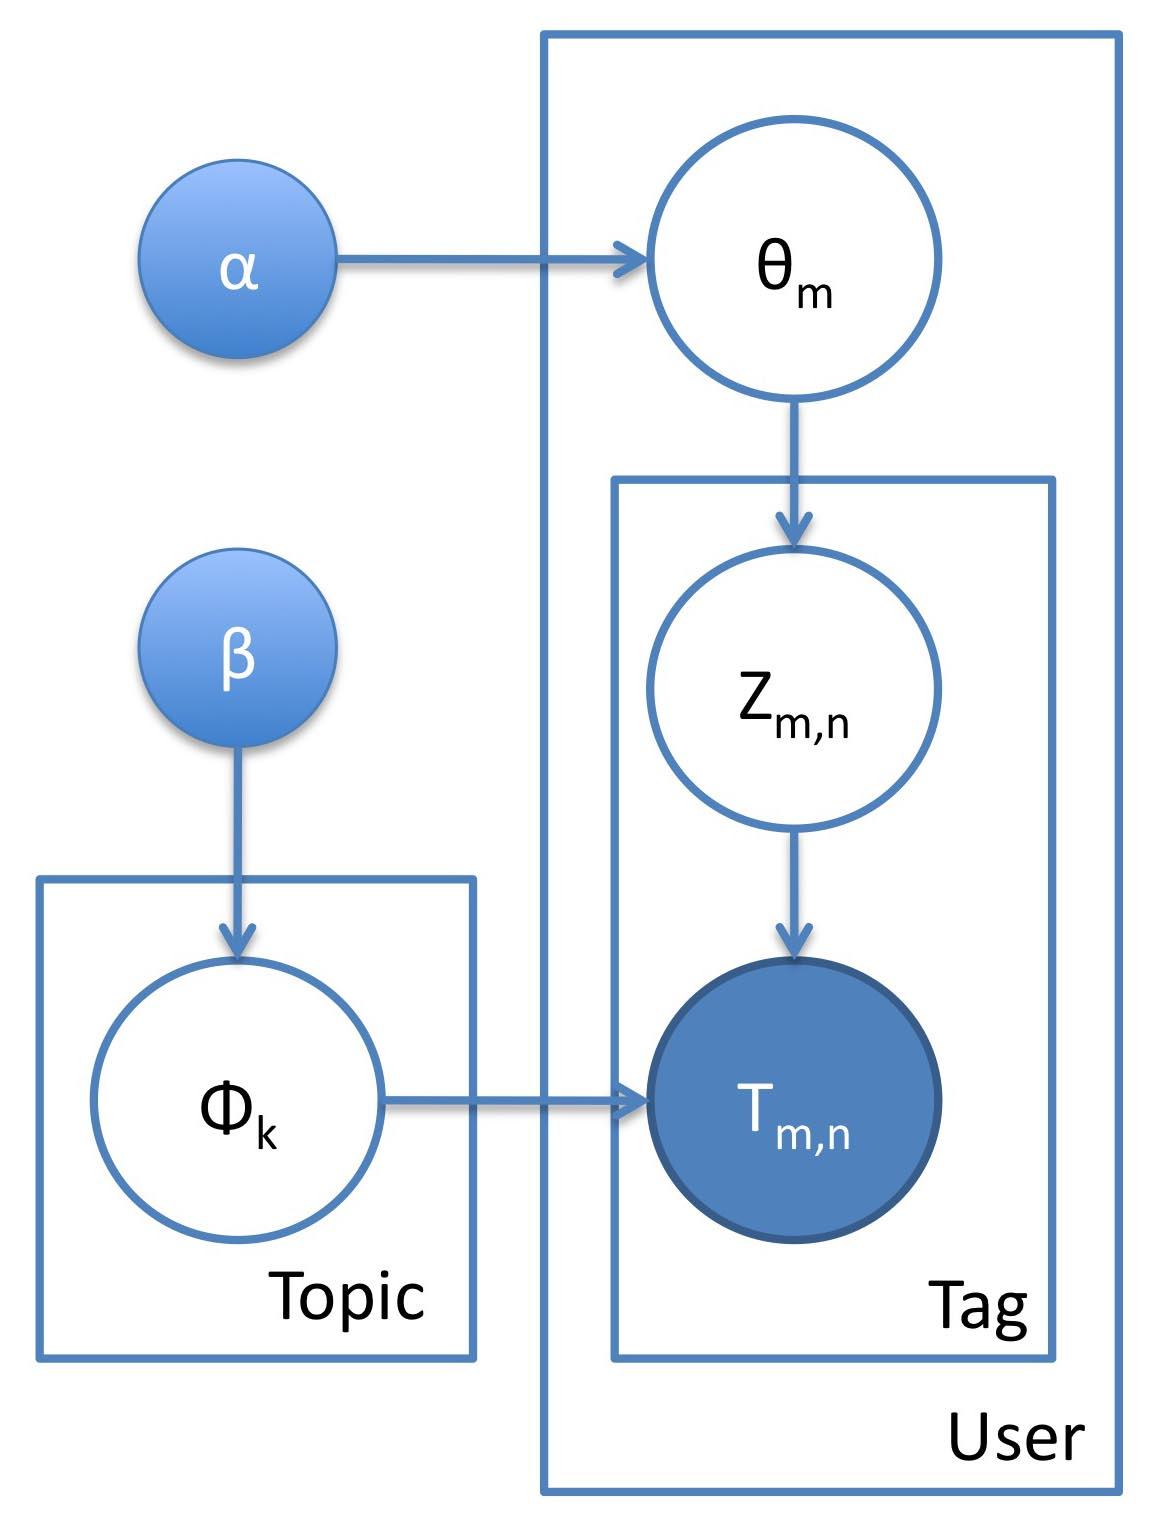
\includegraphics[ width=3.0in]{lda.jpg}  % "pdflatex"
\caption{User-Topic-Tag (LDA) Model}
\label{fig:lda}
\end{figure}

The intuition behind this model is that users choose their topics and that these chosen topics drive the generation of the tags.
The generative process can be summarized as follows:

%TODO : reformat process as code / pseudo algorithm style
\noindent\rule[0.5ex]{\linewidth}{1pt}
\textbf{Process of generating a user's tag list}\\
\noindent \textbf{for} interest k \textbf{in} [1..K]:\\
\indent draw topic tag distribution $\phi(k)$ $\sim$ Dir($\beta$)\\
\noindent \textbf{for} user $m \in [1,M]$:\\
\indent draw a user-topic distribution $\theta(m)$ $\sim$ Dir($\alpha$)\\  
\indent \textbf{for} each tag $n \in$   user $m$'s tag list, where $n~\in~[1,N_m]$, $m~\in~[1..M]$\\
\indent \indent draw topic $z_{m,n}$  $\sim$ Multi($\theta(m)$)\\
\indent \indent draw tag $t_{m,n}$ $\sim$ Multi($\phi(z_{m,n})$)\\ 
\noindent\rule[0.5ex]{\linewidth}{1pt}

\begin{table}[htbp]
\caption{Model parameters}
\label{tab:parameters}
\centering
\begin{tabular}{|c|c|}
\hline
Parameter & Meaning \\
\hline
$M$ & the total number of users\\
\hline
$K$ & the total number of topics\\
\hline
$V$ & the total number of tags\\
\hline
$N_m$ & the total number of tags for user $m$\\
\hline
$\alpha$ & the parameter of the Dirichlet prior on the per-user topic distributions \\
\hline
$\beta$ & the parameter of the Dirichlet prior on the per-topic tag distributions  \\
\hline
$\theta_m$ & the topic distribution for user $m$ \\
\hline
$\phi_k$ & the tag distribution for topic $k$ \\
\hline
$z_{m,n}$ & the topic for $n^{th}$ tag in $m$'s tag list \\
\hline
$t_{m,n}$ & the specified tag in $n^{th}$ position of $m$'s tag list\\
\hline

\end{tabular}
\end{table}

We use the collapsed Gibbs Sampling method~\cite{griffiths2004finding} to sample the hidden variable $z$, then $\theta$ and $\phi$ can both be estimated.
The inference process is as follows.
We iteratively sample the topic indicator $z_{m,n}$ for each answer tag $t_{m,n}$ according to equation \ref{eq:ldasample}. 


\begin{equation}
\begin{split}
p(z_i= z_{m,n} |u=u_m, t=t_{m,n}, Z, U, T_{\neg i}) &\\
\propto \frac{ C_{u_m,\neg i}^{z_{m,n}} + \alpha }{ \sum_{k=1}^K C_{u_m,\neg i}^k + K* \alpha} &\\
\cdot   \frac{ C_{z_{m,n},\neg i}^{t_{m,n}} + \beta }{ \sum_{t=1}^V C_{z_{m,n},\neg i}^t + V* \beta} &\\ 
\end{split}
\label{eq:ldasample}
\end{equation}

\noindent
where $\neg i$ enforces that all the counters used are calculated with tag $t_i$ excluded. $C_{u,\neg i}^k$ is the number of tags acquired by user $u$ assigned to topic $k$, $C_{k,\neg i}^{t}$ is the number of tags $t$ assigned to topic $k$.

Then with a Gibbs sampling, we can estimate $\theta$ and $\phi$ by equation \ref{eq:computetheta} and \ref{eq:computephi}:

\begin{equation}\scriptsize
\theta=\frac{ C_u^k + \alpha}{ \sum_{k=1}^K C_u^k+ K* \alpha}
\label{eq:computetheta} 
\end{equation}
\begin{equation}\scriptsize
\phi =\frac{ C_k^t + \beta}{ \sum_{t=1}^V C_k^t+ V* \beta}
\label{eq:computephi} 
\end{equation}

\noindent
where $C_u^k$ is the number of tags assigned to topic $k$ of user $u$ , $C_k^t$ is the number of tags $t$ assigned to topic $k$.


\section{First experiments: find topics and communities with adapted LDA}
%TODO: FAB: here we are missing details on (1) the dataset characteristics - the dataset of your PhD must be described either at the begining and reference with a unique identifier and reference to the description section if they are used in several chapters OR before the experiment where they are used if they are used only once (2) the implementations, languages, libaries, etc. you used to perform the experiment.

We ran the above described model on a dataset from the popular Q\&A site StackOverflow, each user being represented by her tag list as explained before. We just illustrate some of the results to show the effectiveness of this model.

A first result is the probability for each tag to belong to each topic. This is  shown in Table \ref{tab:ldaresult1}. 
The second result is the probability for a user to belong to different topics of interest. This is shown in Table \ref{tab:ldaresult2}. 
%TODO: FAB: you can add graphical views of these data.

Table \ref{tab:ldaresult1} shows eight examples of the detected topics of interest, each column showing one topic, and the ten rows giving the top 10 tags for each topic, sorted by descending weights. The weight of a tag is the probability of the tag to belong to the topic.  
This table shows that each topic has a clear and focused interest. For example, topic 1 has c-development related tags, topic 2 has java-development related tags, topic 3 has c\#-development related tags, topic 4 has html-development related tags, topic 5 has iphone-development related tags, topic 6 has database related tags, topic 7 has linux-development related tags, topic 8 has non-programming related tags. 
Moreover, weights reflect the relevance of tags to each topic. For example, topic 5 is concerned with iphone-development and its top 3 tags are 'iphone', 'objective-c' and 'cocoa' which are indeed very relevant.
\begin{sidewaystable}
\centering
%\begin{tabular}{|p{40pt}||p{40pt}||p{40pt}||p{40pt}|}
\begin{tabular}{|l|l|l|l|}
\hline
\textbf{topic1} & \textbf{topic2} & \textbf{topic3} & \textbf{topic4} \\
\hline
%\multicolumn{4}{|c|}{c++(0.225), c(0.084), java(0.345), java(0.345), java(0.345), java(0.345), java(0.345), java(0.345), java(0.345), java(0.345)}\\
%\hline
 \textbf{c++}(0.225)& \textbf{java}(0.345)& \textbf{c\#}(0.225)& \textbf{php}(0.117) \\ 
\hline
 \textbf{c}(0.084)& \textbf{eclipse}(0.023)& \textbf{.net}(0.128)& \textbf{javascript}(0.115) \\ 
\hline
 \textbf{windows}(0.020)& \textbf{swing}(0.015)& \textbf{asp.net}(0.059)& \textbf{html}(0.059) \\ 
\hline
 \textbf{stl}(0.014)& best-practices (0.014)& \textbf{vb.net}(0.019)& \textbf{jquery}(0.056) \\ 
\hline
 algorithm(0.014)& multithreading (0.011)& \textbf{linq}(0.018)& \textbf{css}(0.042) \\ 
\hline
 c\#(0.013)& xml(0.010)& windows-forms (0.016)& mysql(0.029) \\ 
\hline
 \textbf{win32}(0.013)& \textbf{spring}(0.010)& \textbf{visual-studio} (0.015)& \textbf{ajax}(0.021) \\ 
\hline
 linux(0.011)& performance (0.009)& \textbf{asp.net-mvc} (0.015)& \textbf{web-development} (0.019) \\ 
\hline
 best-practices (0.011)& jsp(0.008)& wpf(0.012)& regex(0.018) \\ 
\hline
 multithreading (0.011)& generics(0.008)& best-practices (0.011)& \textbf{asp.net}(0.015) \\ 
\hline
\hline
\textbf{topic5} & \textbf{topic6} & \textbf{topic7} & \textbf{topic8} \\
\hline
 \textbf{iphone}(0.137)& \textbf{sql}(0.181)& \textbf{python}(0.181)& subjective(0.143) \\ 
\hline
 \textbf{objective-c} (0.123)& \textbf{sql-server}(0.150)& \textbf{perl}(0.056)& \textbf{best-practices} (0.038) \\ 
\hline
 \textbf{cocoa}(0.080)& \textbf{database}(0.062)& \textbf{regex}(0.031)& \textbf{language-agnostic} (0.035) \\ 
\hline
 ms-access(0.062)& delphi(0.042)& \textbf{linux}(0.030)& programming (0.028) \\ 
\hline
 \textbf{cocoa-touch} (0.056)& \textbf{sql-server-2005} (0.042)& \textbf{ruby}(0.027)& \textbf{not-programming-related} (0.019) \\ 
\hline
 \textbf{iphone-sdk} (0.041)& \textbf{mysql}(0.039)& django(0.023)& \textbf{career-development} (0.018) \\ 
\hline
 vba(0.035)& \textbf{tsql}(0.037)& ruby-on-rails (0.021)& \textbf{learning}(0.017) \\ 
\hline
 excel(0.023)& \textbf{oracle}(0.028)& beginner(0.017)& polls(0.017) \\ 
\hline
 vb6(0.022)& \textbf{database-design} (0.025)& git(0.013)& programming-languages (0.015) \\ 
\hline
 xslt(0.021)& \textbf{stored-procedures} (0.017)& \textbf{bash}(0.013)& \textbf{design}(0.014) \\ 
\hline
\end{tabular}
\caption{Top 10 related tags for detected topics of interest}
\label{tab:ldaresult1}
\end{sidewaystable}

Table \ref{tab:ldaresult2} shows six randomly chosen users and their top 10 tags. The first row contains user ids, the second row contains their detected topics of interest with their probability. The following ten rows show the top 10 tags for each user. We replaced topic ids with topic names which we have assigned to them according to their associated tags.
\begin{sidewaystable}%[htbp]
\centering
%\begin{tabular}{|p{60pt}|p{60pt}|p{60pt}|}
\begin{tabular}{l|l|l}
\hline
user\_21886&user\_14860&user\_15401\\
\hline
\textbf{\textcolor{blue}{html-development}} (0.284)  & \textbf{\textcolor{blue}{c-development}} (0.333) &\textbf{\textcolor{blue}{database-related}} (0.383)\\
 \textbf{\textcolor{brown}{c-development}} (0.275) &  \textbf{\textcolor{brown}{linux-development}} (0.196)& \textbf{\textcolor{brown}{non-programming-related}} (0.290)\\

\hline
python(93)&\textcolor{blue}{c}(152)&\textcolor{blue}{sql-server}(108)\\
%\hline
\textcolor{brown}{c++}(64)&\textcolor{blue}{c++}(148)&\textcolor{blue}{database}(64)\\
%\hline
\textcolor{blue}{javascript}(45)&java(89)&\textcolor{blue}{sql}(63)\\
%\hline
\textcolor{blue}{html}(34)&subjective(89)&\textcolor{brown}{subjective}(45)\\
%\hline
\textcolor{brown}{c\#}(33)&c\#(68)&python(43)\\
%\hline
\textcolor{blue}{css}(32)&sql(68)&\textcolor{blue}{sql-server-2005}(31)\\
%\hline
\textcolor{brown}{visual-studio}(29)&\textcolor{blue}{windows}(67)&\textcolor{brown}{best-practices}(27)\\
%\hline
\textcolor{brown}{windows}(27)&\textcolor{brown}{linux}(54)&.net(25)\\
%\hline
\textcolor{brown}{c}(27)&\textcolor{brown}{bash}(48)&c++(23)\\
%\hline
.net(24)&\textcolor{brown}{regex}(43)&c\#(22)\\
\hline
\hline
user\_78374&user\_53897&user\_23743\\
\hline
\textbf{\textcolor{blue}{non-programming-related}} (0.493)&\textbf{\textcolor{blue}{java-development}} (0.835)&\textbf{\textcolor{blue}{iphone-development}} (0.683)\\
\textbf{\textcolor{brown}{linux-development}} (0.316)&\textbf{\textcolor{brown}{non-programming-related}} (0.075)& \textbf{\textcolor{brown}{non-programming-related}} (0.155)\\

\hline
\textcolor{blue}{subjective}(35)&\textcolor{blue}{java}(366)&\textcolor{blue}{objective-c}(73)\\
%\hline
\textcolor{brown}{python}(32)&\textcolor{blue}{eclipse}(24)&\textcolor{blue}{cocoa}(71)\\
%\hline
\textcolor{blue}{best-practices}(16)&\textcolor{blue}{tomcat}(20)&\textcolor{blue}{iphone}(34)\\
%\hline
c(13)&\textcolor{brown}{subjective}(18)&\textcolor{blue}{cocoa-touch}(21)\\
%\hline
programming(13)&\textcolor{blue}{performance}(18)&\textcolor{blue}{mac}(19)\\
%\hline
c++(10)&\textcolor{brown}{best-practices}(16)&\textcolor{blue}{osx}(17)\\
%\hline
\textcolor{blue}{beginner}(8)&\textcolor{blue}{j2ee}(14)&\textcolor{blue}{iphone-sdk}(13)\\
%\hline
\textcolor{blue}{not-programming-related}(8)&\textcolor{blue}{jar}(13)&\textcolor{blue}{xcode}(10)\\
%\hline
\textcolor{blue}{language-agnostic}(6)&logging(10)&\textcolor{brown}{subjective}(8)\\
%\hline
\textcolor{blue}{coding-style}(5)&c\#(9)&c(8)\\
\hline
\end{tabular}
\caption{Detected topics of interest}
\label{tab:ldaresult2}
\end{sidewaystable}

\section{Discussion: the limitation and problems}
The above experiments verified that, by applying topic models on Q\&A website, we are ideed able to detect overlapping communities, and that the detected topics are meaningful and could be used to explain the shared interest of each corresponding community as in our work, we directly use each topic to represent a community of interest.

However, we found that there are three limitations when applying LDA models to our task:

\begin{itemize}
  \item The first one is a lack of efficiency: the complexity of the probabilistic model was prohibitive.
  %TODO: FAB you should provide details on the computation time, complexity, etc. to make your point
  \item The second limitation is that the  original LDA model does not enable to extract temporal and expertise information. 
  %TODO: FAB explain why i.e. what is missing in the model to achieve that
  \item The third limitation is that the detected probability distributions cannot be compared with each other.
  %TODO: FAB explain why i.e. what noramilization would be required to do that AND why this would be useful
\end{itemize}

Therefore, in the rest of this thesis we extended our work in two directions:

\begin{enumerate}
 \item First, we developed a more simple method to detect topics and overlapping communities to solve the first problem: the TTD method is presented in Chapter \ref{chap:ttd}.
  \item Second, we propose a more complex model to extract more information from user generated content to answer the two other limitations: the TTEA method is presented in Chapter \ref{chap:ttea}.
\end{enumerate}
 
